\chapter{Fazit}
\label{cha:fazit}

\section{Zusammenfassung}

Das Ziel der Abschlussarbeit war die Implementierung einer Software, mit welcher Systemadministratoren sich in Echtzeit über den Status eines administrierten Netzwerkes informieren können. Die Informationsquelle für Abfragen ist die Software Graylog Open, welche Systemprotokolle sämtlicher Geräte in einem Netzwerk zentral sammelt und durchsuchbar macht. Den Administratoren sollte es ermöglicht werden, über eine auf gesprochener Sprache basierende Eingabemöglichkeit Anfragen zu verfassen. Die Aufgabe der zu implementierenden Software ist es, die Informationen aus der über den Messenger Telegram gesendeten Sprachnachricht zu extrahieren und damit eine Anfrage an Graylog zu stellen. Schließlich sollte die Software die Antwort von Graylog ebenfalls in einer Sprachnachricht an den Benutzer zurücksenden. 

Die Implementierung der Software verlief planmäßig, sodass die gestellten Anforderungen erfüllt werden konnten. Während der Entwicklung und bei der Prüfung erster Prototypen fiel auf, dass die nicht-funktionalen Anforderungen Verarbeitungsgeschwindigkeit und Erkennungsgenauigkeit der Spracherkennung an ein Produkt, welches ausschließlich per Sprache bedient werden soll hohe Ansprüche an die Qualität der Implementierung stellen. Durch die Verwendung von asynchronen Funktionen konnte die Verarbeitungsgeschwindigkeit erheblich reduziert werden. Eine weitere Funktion, welche zur Verbesserung der Erkennungsgenauigkeit beigetragen hat, waren die implementierten Aliasdefinitionen. Mit diesen konnte die im Gegensatz zur Transkription von alltäglicher Sprache niedrige Treffergenauigkeit von Fachbegriffen aus dem Bereich der Informatik gut kompensiert werden. 

Auch aus Sicht der IT-Sicherheit bringt die Verwendung des Telegram-Bots Vorteile gegenüber der Verwendung der Graylog Webschnittstelle, sofern der Zugriff von außerhalb des Netzwerks erfolgt. Die Graylog-Instanz sammelt die Systemprotokolle sämtlicher Geräte im Netzwerk und ist damit ein besonders schützenswertes System in einem Firmennetzwerk. Der Zugriff von außerhalb sollte gut abgesichert werden. Es existieren mehrere Möglichkeiten, um webbasierte Systeme aus einem internen Netzwerk über das Internet erreichbar zu machen. Eine simple Möglichkeit besteht darin, auf dem Internetrouter eine Portweiterleitung einzurichten. Besser ist jedoch eine Veröffentlichung über einen 'reverse proxy'. Ein Proxy ist ein System, welches stellvertretend für ein weiteres System eine Kommunikation mit dem gewünschten Partner übernimmt. Häufig werden Proxies in Firmennetzwerken für die Filterung von besuchten Internetseiten eingesetzt. Dabei wendet sich ein PC im internen Netzwerk an den Proxyserver und fragt eine Internetressource an. Der Proxy agiert als Vermittler und bezieht die Internetressource, bevor er diese an den PC weiterleitet. Bei einem reverse proxy ist das Prinzip umgekehrt. Hier übernimmt der Vermittler die Kommunikation von Geräten außerhalb eines Netzwerks (beispielsweise dem Internet) stellvertretend für die Quelle und kontaktiert den gewünschten Verbindungspartner im internen Netzwerk. Der Vorteil eines reverse proxies gegenüber einer Portweiterleitung besteht darin, dass die HTTP-Anfragen detailliert bearbeitet, gefiltert und protokolliert werden können. Bestimmte Adressmuster, welche für Angriffe verwendet werden können so beispielsweise direkt blockiert werden. Der alleinige Einsatz eines reverse proxies mit Filter für die Veröffentlichung über das Internet reicht bei einem schützenswerten System nicht aus. Daher wird häufig eine HTTP-Authentifizierung zwischengeschaltet, welche durch die Anforderung von vom Ziel unabhängigen Zugangsdaten eine zusätzliche Sicherheitsebene schafft. Ein reverse proxy mit auf die Zielapplikation abgestimmten Filtermechanismen sowie einer zusätzlichen Authentifizierungsschicht bietet ausreichenden Schutz für eine Veröffentlichung im Internet. Der Einsatz eines solchen reverse proxies mit Graylog ist jedoch nicht möglich, da Graylog nicht kompatibel zu Anfragen mit HTTP-Authentifizierung ist \footnote{Fehlerbericht und Erweiterungsvorschlag eines Anwenders, welcher Graylog über einen reverse proxy mit HTTP-Authentifizierung erreichbar machen möchte: \url{https://github.com/Graylog2/graylog2-server/issues/6831}}. Eine Alternative zum reverse proxy bietet ein Dienst, welcher die Funktion eines proxies oder Stellvertreters für die Verbindung zur Graylog-Webschnittstelle schafft. Dieser Dienst kann für beliebige Funktionen implementiert werden, welche über die Graylog REST-API Daten beziehen und weiterverarbeiten. Die in dieser Abschlussarbeit implementierte Software ist ein Beispiel für einen solchen Vermittler auf Applikationsebene.

\begin{figure}[h!]
\centering
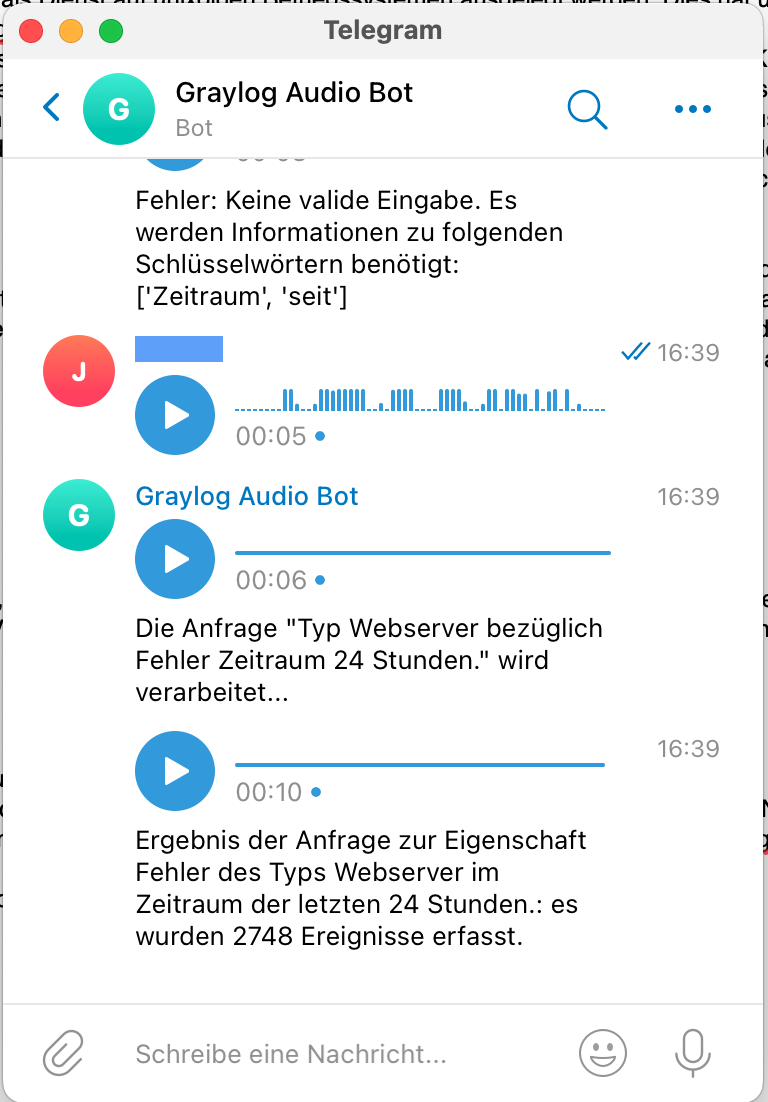
\includegraphics[scale=0.7]{bsp-betrieb}
\caption{Bot beantwortet eine Anfrage in Telegram für macOS.}
\end{figure}

\begin{figure}[h!]
\centering
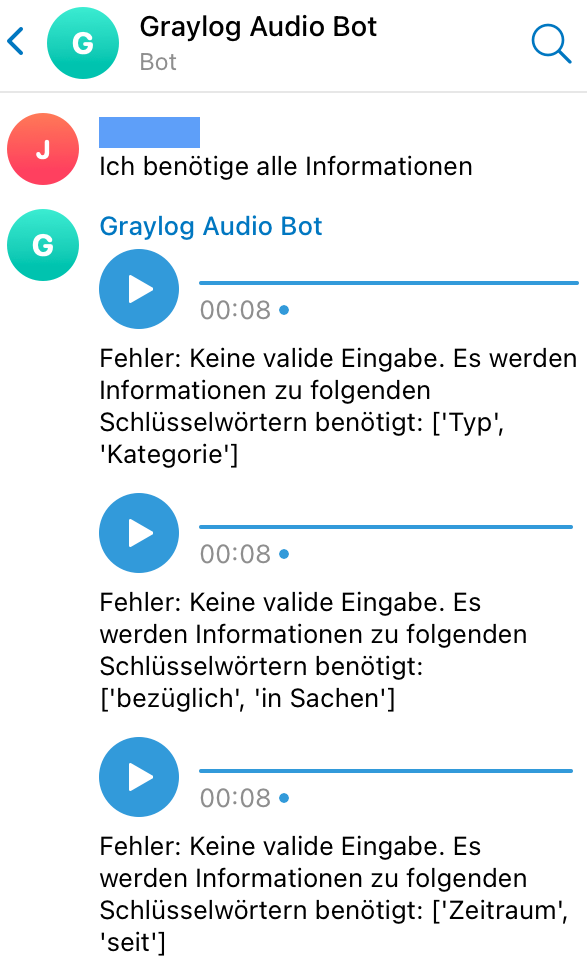
\includegraphics[scale=0.7]{bsp-fehler}
\caption{Bot reagiert auf fehlerhafte Anfrage in Telegram für macOS.}
\end{figure}

\section{Ausblick}

